% !Mode:: "TeX:UTF-8"
% !TEX program  = xelatex
\newgeometry{margin=1.6in, marginpar=1.5in}

\title{Geometric Progression and Sum}
\author{}
\date{}

\maketitle



\begin{abstract}
    We present a concise formula for the sum of the first $n$ terms in a geometric progression, which is easy to implement. And we put it forward to the infinite case. This new method is more efficient and well-performed.
\end{abstract}
\paragraph{Keywords:} geometric progression, summation



\section{Introduction}\label{S:introduction}
Historically, geometric series played an important role in the early development of calculus, and they continue to be central in the study of convergence of series. Geometric series are used throughout mathematics, and have important applications in physics, engineering, biology, economics, computer science, queueing theory, and finance. The intuitive method to calculate the sum of the first $n$ terms of a geometric progression is adding them one by one. It can be sophisticated when $n$ is very large. This is a right but clumsy method, so an easier one is needed. 

We use the misalignment subtraction to develop the formula to solve this problem. And we apply our method to three examples. Comparing with the traditional one, the calculation is extremely simple. The ratio of any two successive terms in the geometric progression is a constant, we call it common ratio and denote it as $q$. A geometric series only depends on its first term $a$ and common ratio $q$. The formula for the sum of the first $n$ terms $S_n$ is:
\begin{equation*}
    S_n = \begin{cases}
        na & (q=1) \\
        \frac{{a\left(1-q^{{n}}\right)}}{{1-q}} & (q\neq 1)
        \end{cases}
\end{equation*}
This series is converge and equals to $\frac{{a}}{{1-q}}$ when $|q|<1$.

The present paper is built up as follows. In Section~\ref{S:introduction}, we  we introduce the background of the geometric progression. Section~\ref{S:geometric-series} is about the definition of the geometric progression and the common ratio. We devote Section~\ref{S:summation-formula} to the construction of the formula, the derivation is presented and its proposals are given. In Section~\ref{S:applications}, we apply our method to two numerical examples and one economic example. Conclusions and discussions are presented in Section~\ref{S:conclusions-and-discussions}.



\section{Geometric Series}\label{S:geometric-series}
\subsection{Definition}
\begin{figure}[h]
    \centering{
    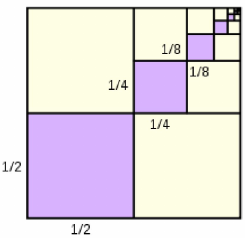
\includegraphics[width=0.4\textwidth]{figures/geometric_progression-1}}
    \caption{Squares(source: wikipedia)}\label{F:geometric-progression}
\end{figure}

In mathematics, a geometric series is a series with a constant ratio between successive terms. For example, the series 
\begin{equation*}
    \frac{1}{2}+\frac{1}{4}+\frac{1}{8}+\frac{1}{16}+\cdots
\end{equation*}
is geometric, because each successive term equals to the previous one multiply $\frac{{1}}{{2}}$. Geometric series are among the simplest examples of infinite series with finite sums, although not all of them have this property. 
The following table shows several geometric series with different start terms and common ratios:
\begin{equation*}
    \begin{aligned}
        & 2, 20, 200, 2000, \cdots \\
        & 2, 4, 8, 16, \cdots \\
        & 3, 9, 27, 81, \cdots 
    \end{aligned}
\end{equation*}



\section{Summation Formula}\label{S:summation-formula}
The sum of a geometric series is finite when $|q|<1$; as the numbers near zero, it becomes insignificantly small, allowing to be calculated despite the series contain infinitely terms. We can use the self-similarity of the series to compute the sum.
\subsection{Derivation of the Formula}
Let $a$ and $q$ be two constants. Consider an infinite sequence of numbers
\begin{equation}\label{E:sequence}
    a_1, a_2, a_3, \ldots
\end{equation}
where the $i$th term in this sequence is
\begin{equation}\label{E:ith-term}
    a_i = a_1 q^{(i-1)}, \quad (i=1,2,3,\ldots)
\end{equation}
for $i=1,2,3\cdots$. The sum of the first $n$ terms of the sequence in Equation~\eqref{E:sequence} is denoted by $S_n$ : that is,
\begin{equation*}
    S_n = a_1 + a_2 + \cdots + a_n.
\end{equation*}

We are interested in finding the value of $S_n$ for any given $n$.

A direct approach is to first compute the $n$ terms ${a_1,a_2,\cdots,a_n}$ through Equation~\eqref{E:ith-term}, and then add them up to obtain the value, but this is clearly time-consuming when $n$ is large. We show an efficient formula below, which expresses the $S_n$ as a simple function of $a$, $q$ and $n$. Since
\begin{equation}\label{E:summation-expression-1}
    S_n = a + aq^1 + \cdots + aq^{(n-1)},
\end{equation}
multiplying $q$ of the both sides of the Equation~\ref{E:summation-expression-1}, we obtain
\begin{equation}\label{E:summation-expression-2}
    \begin{aligned}
        qS_n &= q(a + aq^1 + \cdots + aq^{(n-1)}) \\
             &= aq^1 + aq^2 + \cdots + aq^n
    \end{aligned}
\end{equation}
Subtract $S_n$ from both sides of the Equation~\eqref{E:summation-expression-2}, we obtain
\begin{equation}\label{E:summation-expression-3}
    (q-1)S_n = aq^n - a.
\end{equation}
If $q\neq 1$, dividing both side of Equation~\eqref{E:summation-expression-3} by $(q-1)$, we obtain
\begin{equation*}
    S_n = \frac{a(1-q^n)}{1-q},
\end{equation*}
which holds for any integer $n$.

If $q = 1$,we can easily get that $S_n = na$.

Till now, we finish the derivation of the formula. We can find that the result is concise and can be easily employed.


\subsection{Extensions of the Formula}
We derivate the sum of the fist $n$ terms of a geometric sequence. What will happen when the $n$ is extended to infinite? Without loss of generality, we assume $a>0$.

If $q=1$, then
\begin{equation*}
    S = \lim_{n\to\infty} S_n = \lim_{n\to\infty} na = \infty;
\end{equation*}

If $-1<q<1$, then $\lim_{n\to\infty}q^n=0$, we obtain
\begin{equation*}
    S = \lim_{n\to\infty} S_n = \frac{a}{1-q};
\end{equation*}

If $q>1$ or $q<-1$, this series does not converge, $\left| S \right| = \mathop {\lim }\limits_{n \to \infty } \left| {{S_n}} \right| = \infty$.

Till now, we have finished the extended of the formula and we have found that the new method performs well even when $n$ tends to infinity.



\section{Applications}\label{S:applications}
\subsection{Numerical Examples}
Some numerical experiments have been carried out in this section.

\paragraph{Example 1:} Calculate $1/2+1/2^2+\cdots+1/2^{20}$.

Using the formula above, we can easily find that
\begin{equation*}
    S_{20} = \frac{\frac{1}{2}\left(1-\frac{1}{2^{20}}\right)}{1-\frac{1}{2}} = 1 - \frac{1}{2^{20}}.
\end{equation*}

But if we calculate it by the traditional method, we need to add 19 times one by one. You can easily find that the new method is more efficient. 

\paragraph{Example 2:} Calculate $1/2+1/2^2+\cdots$.

Using the formula above, we can easily find that
\begin{equation*}
    \begin{aligned}
        S_{n} &= \frac{\frac{1}{2}\left(1-\frac{1}{2^{n}}\right)}{1-\frac{1}{2}} = 1 - \frac{1}{2^{n}}. \\
        S &= \lim_{n\to\infty} S_n = 1.
    \end{aligned}
\end{equation*}

But if we calculate it by the traditional method, we will find that may not be useful, because we can never finish this job to add up all terms.


\subsection{Economic Example}
In economics, geometric series are used to calculate the value of an annuity (a sum of money to be paid in regular intervals). We present an economic example which is from wikipedia. 

Suppose $\$100$ will be paid to the owner of the annuity once per year (at the end of the year) in perpetuity. Receiving $\$100$ a year from now is worth less than an immediate $\$100$, because one cannot invest the money until he receives it. In particular, the present value of $\$100$ one year later is $\frac{{\$100}}{{1 + I}}$, where $I$ is the yearly interest rate. Similarly, two years later, the payment of $\$100$ has a present value of  $\frac{{\$100}}{{(1 + I)}^2}$ (squared because two years'worth of interest is lost by not receiving the money right now). Therefore, the present value of receiving $\$100$ per year in perpetuity is:
\[
    \sum_{n=1}^\infty  {\frac{{\$100}}{{{{\left( {1 + I} \right)}^{n }}}}}  = \frac{{\$100/\left( {1+I} \right)}}{{1 - 1/\left( {1 + I} \right)}} = \frac{{\$100}}{I}
\]

If the yearly interest rate is $10\%(I=0.10)$, then the entire annuity has present value of $\$100/0.10=\$1000$.

This sort of calculation is used to compute the APR of a loan (such as a mortgage loan). It can also be used to estimate the present value of expected stock dividends, or the terminal value of a security.



\section{Conclusions and Discussions}\label{S:conclusions-and-discussions}
In this paper, we present a formula to get the sum of the finite geometric progression and put it forward to the infinite cases. the formula is developed by misalignment subtraction. The examples evidently demonstrate that the formula is efficient for computing $S_n$, as it does not require to add the terms one by one.  It can be used for any geometric sequences even when $n$ is infinite, while the traditional method performs badly. 

This formula is the foundation of many other jobs. It is efficient and basic to solve many problems in our lives.



\section*{Acknowledgement}
My deepest gratitude goes first to the Professor Wang and Dr Zhang, for their guidance and teaching about how to write a paper and use the \LaTeX. I owe my sincere gratitude to my parents because they support me for every decision. I thank my advisor Professor He, he gives a lot help to my study. Then, I thank my group members because they give me some suggestions about this paper.



\begin{thebibliography}{9}
    \bibitem{tang2013} 汤涛, 丁玖. 数学之英文写作[M]. 北京: 高等教育出版社, 2013.
    \bibitem{highham1998} HIGHAM N J. Handbook of writing for the mathematical sciences[M]. Philadelphia: Society for Industrial and Applied Mathematics, 1998.
\end{thebibliography}
